% !Tex root = e4_tp1_ej1
\documentclass[e4_tp1_main.tex]{subfiles}

\begin{document}

\begin{wrapfigure}[11]{R}{0.4\textwidth}
  \centering
  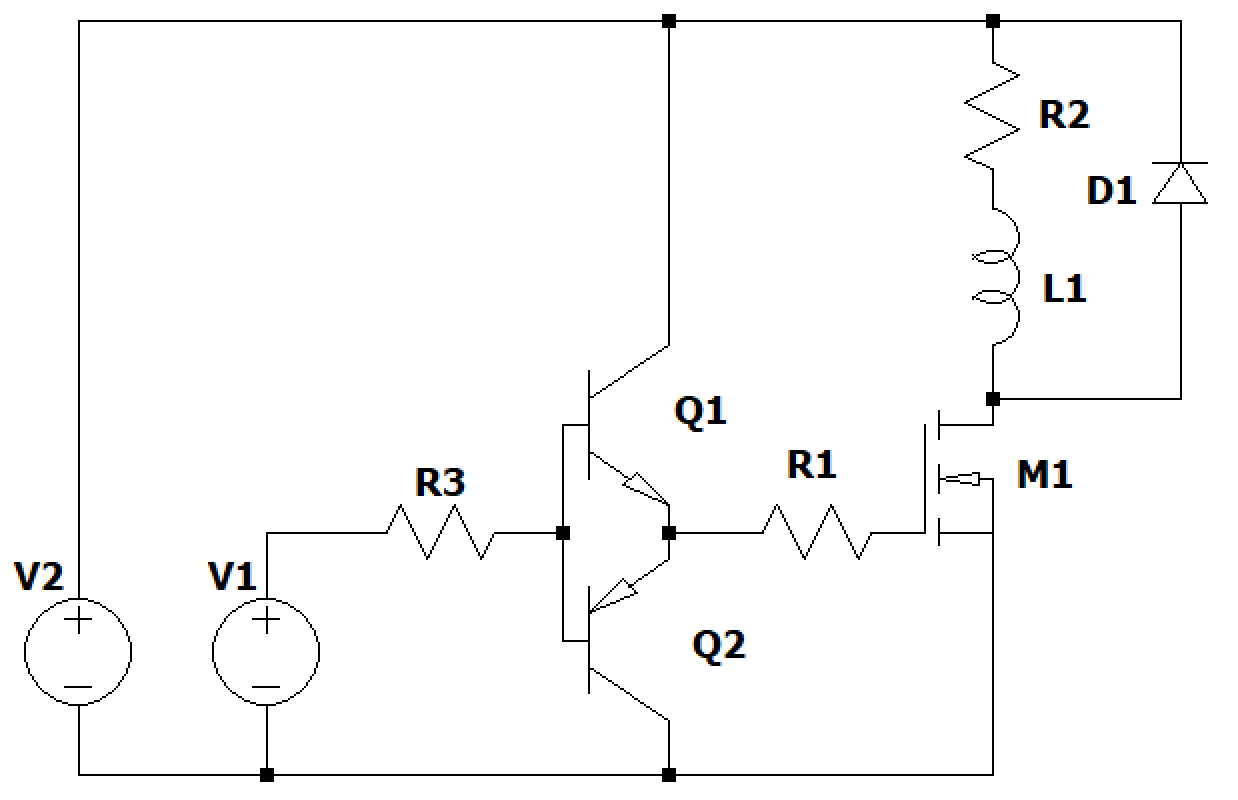
\includegraphics[width=\linewidth]{images/ej1/circuit_1.png}
  \caption{Circuito para análisis de disparo de transistor MOSFET}
  \label{fig:circuit_1}
\end{wrapfigure}
\section{Ejercicio 1}


Se procederá al análisis del circuito de la \autoref{fig:circuit_1}. El mismo es un circuito destinado al análisis del disparo de un transistor MOSFET.


\subsection{Carga Inductiva}
La carga inductiva tiene dos valores de corriente, uno cuando se prende el MOSFET ($I_0$), y otro cuando se apaga ($I_1$). Siendo $t_1 = D/f_s$, $t_2 = (1-D)/f_s$, $\tau_{RL}=L/R$, $f_s$ la frecuencia del switch y $D$ el duty cycle, entonces resolviendo el circuito RL se tiene que
\begin{flalign*}
I_0 &= \frac{V_2}{R_2}\frac{1-exp(-t_1/\tau_{RL})}{\exp(t_2/\tau_{RL})-\exp(-t_1/\tau_{RL})} &\\
I_1 &= \frac{V_2}{R_2}\frac{(1-\exp(-t_1/\tau_{RL}))\exp(t_2/\tau_{RL})}{\exp(t_2/\tau_{RL})-\exp(-t_1/\tau_{RL})}
\end{flalign*}%


\subsection{Conmutación MOSFET}

Durante la conmutación del MOSFET, se cargan y descargan capacidades internas. Las capacidades a considerar en en análisis de conmutación son la Capacidad Gate-Source $C_{GS}$ y la capacidad Gate-Drain $C_{GD}$.

\begin{wrapfigure}[20]{R}{0.4\textwidth}
  \centering
  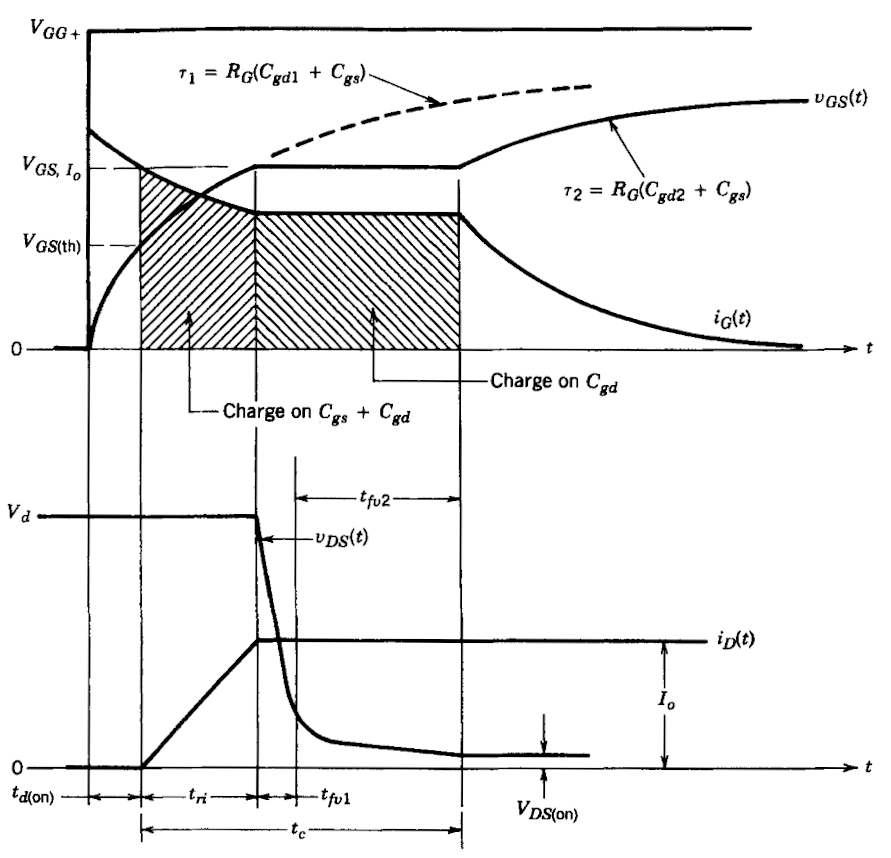
\includegraphics[width=\linewidth]{images/ej1/theory_mosfet.png}
  \caption{Curvas de tensión y corriente en el MOSFET durante el encendido}
  \label{fig:mosfet_theory}
\end{wrapfigure}
\subsubsection{Encendido del MOSFET}




Considerando que, ante un escalón de tensión en provisto por el circuito Driver, dichas capacidades comienzan a cargarse, se puede modelar la primera etapa del prendido del MOSFET con un circuito RC, por lo que la tensión $V_{G}$ en función del tiempo puede ser aproximada por $V_G(t) = V_1 (1-\exp(-t/\tau_1))$, donde $\tau_1 = R_1\tilde{C}_{G,1}$ y $\tilde{C}_{G,1} = C_{GS} + C_{GD,1}$. Cuando la tensión en el Gate llega a $V_{GS,th}$ (en $t=t_{d,on}$), comienza a formarse la capa de inversión, por lo que la corriente del Drain $I_D$ comienza a aumentar hasta llegar al valor $I_0$ impuesto por la carga inductiva y hasta que el diodo deje de conducir (en $t=t_1$). Esto ocurrirá cuando la tensión en el Gate llegue a un valor $V_G=V_{G,I_D=I_0}$. El tiempo entre que comienza a circular corriente hasta que se alcanza el valor $I_0$ se denomina $t_{ri}$. Se puede demostrar que $t_{d,on} = -\tau_1 \ln\left(1-V_{G,th}/V_1\right)$, $t_{1} = -\tau_1 \ln\left(1-V_{G,I_D=I_0}/V_1\right)$ y $t_{ri} = t_{1} - t_{d,on}$.


Luego, cuando la corriente de Drain llega al valor $I_0$, el valor de la tensión en el Gate se mantiene temporalmente en $V_G=V_{G,I_D=I_0}$, por lo que la capacidad $C_{GS}$ deja de cargarse, mientras se sigue cargando $C_{GD}$ a corriente constante. A medida se cargue $C_{GD}$ se formará la capa de acumulación, bajando la resistencia $R_{DS}$, por lo que disminuye la tensión $V_{DS}$ hasta alcanzar el valor $V_{DS,on}$. Dado que la capacidad $C_{GD}$ varía durante este proceso, pues varían la longitud de la capa de acumulación, suele utilizarse el valor de la carga total $\Delta Q$ para estimar la duración de esta etapa. Con esto, el tiempo que transcurre desde que empieza a caer la tensión $V_{DS}$ hasta que alcanza el valor $V_{DS,on}$ puede estimarse según $t_{fv} = \Delta Q/I_{G,on} = (\Delta Q R_1)/(V_{1}-V_{G,I_D=I_0})$. A lo largo de esta etapa, cambia el valor de $C_{GD}$ de $C_{GD,1}$ a $C_{GD,2}$. El cambio de la tensión $V_{DG}$ en función del tiempo puede expresarse según $\frac{dV_{DG}}{dt} = \frac{V_{GG}-V_{G,I_D=I_0}}{R_1C_{GD}}.$

Una aproximación es considerar que esto ocurre en dos etapas: una donde $C_{GD} = C_{GD,1}$ y otra donde $C_{GD} = C_{GD,2}$. Luego, la tensión en el Gate sigue creciendo hasta llegar al valor $V_{GG}$. El tiempo característico asociado está dado por $\tau_2 = R_1\tilde{C}_{G,2}$, donde $\tilde{C}_{G,2} = C_{GS} + C_{GD,2}$. Un gráfico esquemático mostrando la conmutación del MOSFET se muestra en la \autoref{fig:mosfet_theory}.




\subsubsection{Apagado del MOSFET}

El apagado del MOSFET es similar al encendido, pero en orden contrario. Primero, se comienzan a descargar las capacidades internas por el Gate, por lo que la tensión del Gate en la primera etapa está dada por $V_G(t) = V_{GG} \exp(-t/\tau_2)$. Esto ocurrirá hasta que la tensión $V_G$ alcance el valor $V_{G,I_D=I_0}$ en $t=t_{d,off}$. Puede demostrarse que $t_{d,off}= -\tau_2\ln\left((V_{G,I_D=I_0})/(V_{GG})\right)$. Luego, la tensión en el Gate permanecerá constante mientras se descarga $C_{GD,2}$ a corriente constante durante un tiempo $t_{rv}$. Análogo al caso de encendido, este tiempo está dado por $t_{rv} = \Delta Q/I_{G,off} = (\Delta Q R_1)/(V_{G,I_D=I_0})$

Notar que, al igual que durante el prendido, la capacidad $C_{GD}$ cambia de valor durante este proceso. La misma aproximación en dos etapas aplica para este caso. Finalmente, la tensión en el Gate baja según la ecuación $V_{G} = V_{G,I_D=I_0}\exp(-t/\tau_1)$.

A medida que la tensión cae, comienza a deshacerse el canal formado, por lo que baja el valor de $I_D$ hasta hacerse nulo cuando $V_G=V_{G,th}$. Esto ocurre luego de un intervalo $t_{fi}= -\tau_1\ln\left((V_{G,th})/(V_{G,I_D=I_0}\right)$.

\subsection{Diodo}
\begin{wrapfigure}[20]{R}{0.5\textwidth}
  \centering
  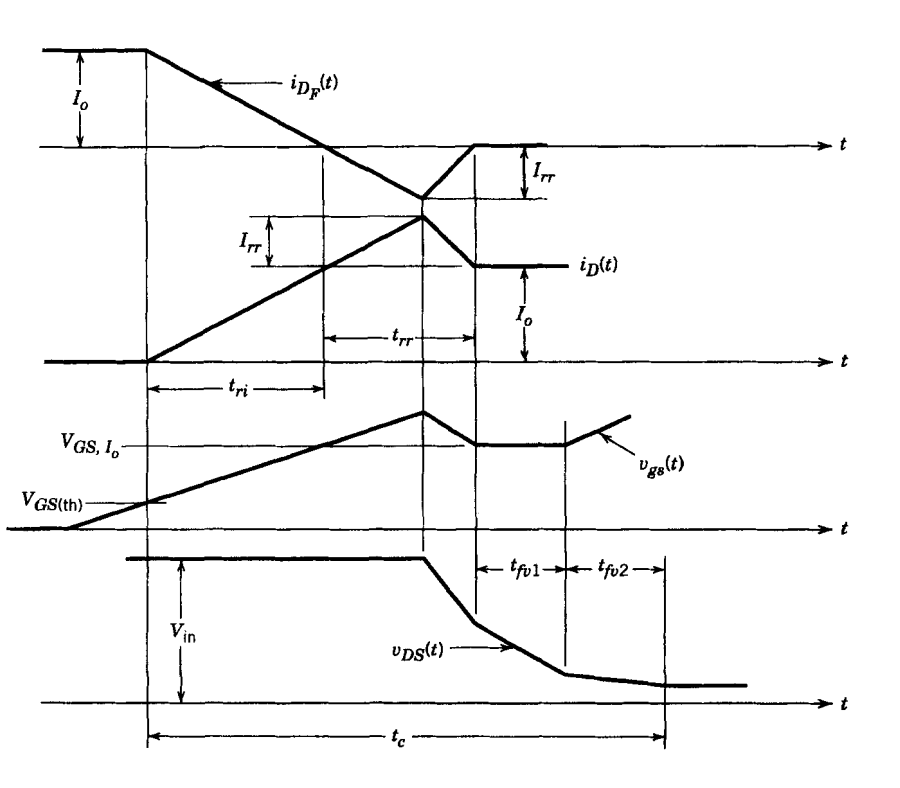
\includegraphics[width=\linewidth]{images/ej1/diode_irr.png}
  \caption{Efectos de $I_{rr}$ en el encendido del MOSFET.}
  \label{fig:mosfet_irr}
\end{wrapfigure}
$ $ %PARA QUE SE PONGA ACÁ

Resulta importante tener en cuenta los efectos de un diodo real en las curvas de conmutación del MOSFET. Al no ser este análisis requisito de este ejercicio, no se realizará un análisis en detalle, pero si se comentará para poder explicar lo observado en simulaciones con un diodo real.

Al apagar el diodo, la corriente sobre el mismo baja, pero como las junturas no se vuelven a formar inmediatamente (los portadores de carga libres deben ser removidos para que la juntura llegue al equilibrio térmico antes de que la misma pueda ser polarizada en inversa), por un cierto tiempo $t_{rr}$ la corriente en el diodo se vuelve negativa hasta llegar a un valor pico $I_{rr}$, y esta corriente puede alcanzar valores significativos.

\subsubsection{Efecto de $I_{rr}$ en la conmutación del MOSFET}
\label{subsubsec:irr_effect}
Por causa de la corriente $I_{rr}$, la corriente de Drain $I_D$ crece hasta el valor $I_0+I_{rr}$, por lo que el valor de $V_{G}$ crece por arriba de $V_{G,I_D=I_0}$. Cuando el diodo se recupera y la corriente vuelve a cero (y, por lo tanto, la corriente $I_D$ baja a $I_0$), el valor de $V_G$ baja a $V_{G,I_D=I_0}$, y el cambio de tensión provee corriente adicional a la capacidad $C_{GD}$, produciendo que $V_{GD}$ y $V_{DS}$ decrezcan rápidamente durante este intervalo de recovery. Los efectos de la corriente $I_{rr}$ en la conmutación del MOSFET pueden observarse en la \autoref{fig:mosfet_irr}. Esta corriente no se tendrá en cuenta para el análisis teórico.

\subsection{Valores de los componentes y variables}

Los valores de los componentes y las variables se muestran en la \autoref{tab:values_1}.

\begin{table}[H]
\centering
\begin{tabular}{|c|c|}
\hline
Parámetro & Valor \\
\hline
$V_0$ (on) & $15$ V \\
\hline
$V_0$ (off) & $0$ V \\
\hline
$f_s$ & $50$ KHz \\
\hline
$D$ (Duty Cycle) & $50\%$ \\
\hline
\end{tabular}
\hspace{0.02\textwidth}
\begin{tabular}{|c|c|c|c|c|c|}
\hline
Componente & $Q_1$ & $Q_2$ & $R_1$ & $R_2$ & $R_3$ \\
\hline
Valor & BC337-25 & BC557B & 100 $\Omega$ & 15 $\Omega$ & 1 $K\Omega$ \\
\hline
Componente & $M_1$ & $L_1$ & $D_1$ & $V_2$ & $V_1$\\
\hline
Valor & IRF530 & 220 $\mu H$ & MUR460 & 50 V & Ver Tabla izq.\\
\hline
\end{tabular}
\caption{Valores de los componentes utilizados.}
\label{tab:values_1}
\end{table}

\subsection{Búsqueda de parámetros en datasheet y cálculo de valores}

Los valores de los parámetros del circuito obtenidos a partir del datasheet del transistor y los valores calculados de las capacidades internas, asi como también los tiempos teóricos de conmutación se muestran en la \autoref{tab:obtained_values_1}.

\begin{table}[H]
\centering
\begin{tabular}{|c|c|c|c|c|c|c|c|c|c|}
\hline
Variable & $I_{0_{off}}$ & $I_{0_{on}}$ & $V_{G,th}$ & $V_{G,I_D=I_{0_{off}}}$   & $V_{G,I_D=I_{0_{on}}}$ & $\tilde{C}_{G,1}$ & $\tilde{C}_{GD,2}$ & $\Delta Q$  \\
\hline
Valor & 2,21 A & 1,12 A & 4 V & 4,8 V & 4,5 V & 650 pF & 1120 pF & 7 nC\\
\hline
\end{tabular}
\\
\begin{tabular}{|c|c|c|c|}
\hline
Variable & $C_{gd,1}$ & $C_{gd,2}$ & $C_{gs}$\\
\hline
Valor & 50 pF & 520 pF & 600 pF\\
\hline
\end{tabular}
\\
\begin{tabular}{|c|c|c|c|c|c|c|c|c|}
\hline
Variable & $t_{d,on}$ & $t_{ri}$ & $t_{fv}$ & $t_{d,off}$ & $t_{rv}$ & $t_{fi}$  \\
\hline
Valor & $21.32$ ns & $3.23$ ns & $71.43$ ns & $127.62$ ns & $145.83$ ns & $11.85$ ns\\
\hline
\end{tabular}	
\caption{Valores obtenidos del datasheet}
\label{tab:obtained_values_1}
\end{table}

\subsection{Curvas teóricas}
Las curvas obtenidas a partir de la teoría se muestran en la \autoref{fig:teoria}.

\begin{figure}[h]
  \centering
  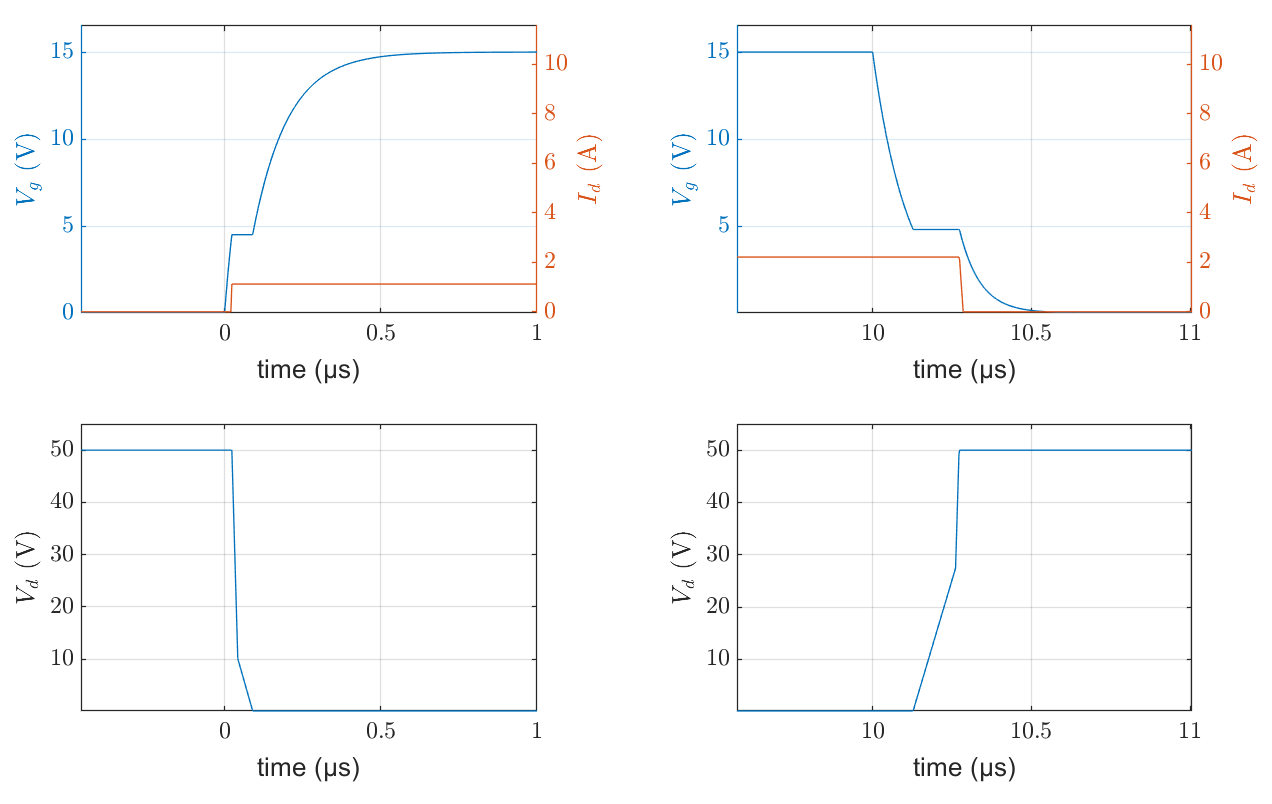
\includegraphics[width=\linewidth]{images/ej1/curvas_teoria.png}
  \caption{Curvas teóricas de $V_G$, $V_{DS}$ e $I_D$.}
  \label{fig:teoria}
\end{figure}


\subsection{Curvas Simuladas y valores obtenidos con la simulación}
Las curvas de conmutación obtenidas en la simulación pueden observarse en la \autoref{fig:simulation}. Los valores de los tiempos de conmutación obtenidos a partir de la simulación se muestran en la \autoref{tab:conmutation_times_simulation}
\begin{table}[H]
\centering
\begin{tabular}{|c|c|c|c|c|c|c|c|c|}
\hline
Variable & $t_{d,on}$ & $t_{ri}$ & $t_{fv}$ & $t_{d,off}$ & $t_{rv}$ & $t_{fi}$  \\
\hline
Valor & $28$ ns & $12$ ns & $183$ ns & $170$ ns & $450$ ns & $13$ ns\\
\hline
\end{tabular}	
\caption{Tiempos de conmutación obtenidos a partir de la simulación.}
\label{tab:conmutation_times_simulation}
\end{table}

\begin{figure}[h]
  \centering
  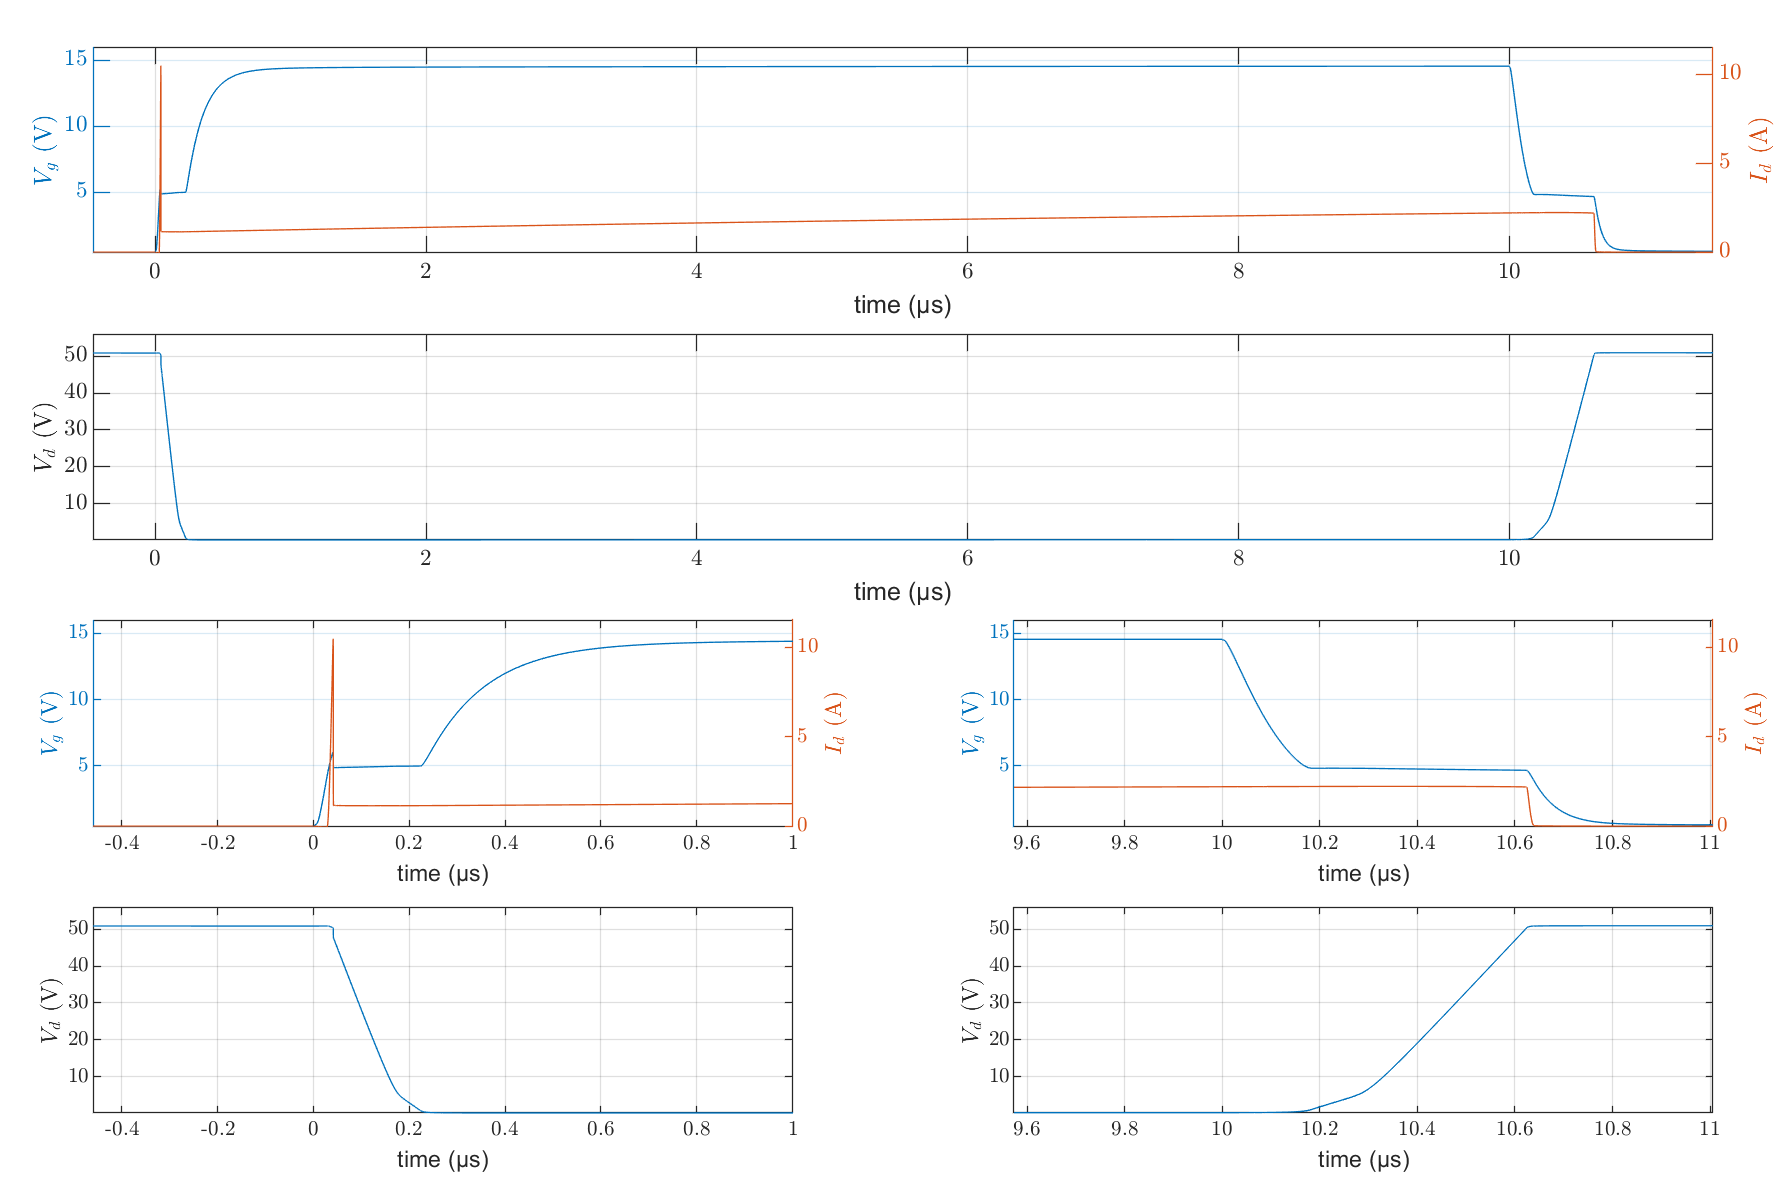
\includegraphics[width=0.7\linewidth]{images/ej1/curvas_simuladas.png}
  \caption{Curvas simuladas de $V_G$, $V_{DS}$ e $I_D$, y detalle de conmutación de encendido y apagado.}
  \label{fig:simulation}
\end{figure}

\subsection{Comparación de resultados obtenidos}
Al comparar los resultados teóricos y las simulaciones, la diferencia más significativa es el pico de corriente que aparece en la corriente de Drain $I_D$. Este pico es debido a la corriente $I_{rr}$ desarrollada en la \autoref{subsubsec:irr_effect}. Este efecto no fue considerado para graficar las curvas teóricas, pero los resultados obtenidos en la simulación ($I_{D,max}=10.29A$, cuando $I_0 = 1.15A$) muestran la importancia de tener en consideración este análisis.

Con respecto a la forma de las curvas obtenidas, las curvas teóricas y simuladas resultan semejantes en forma, con desviaciones por la aproximación del modelo teórico con respecto al modelo de la simulación, presentando algunas diferencias en los tiempos de las distintas etapas de la conmutación. 


Los tiempos de las distintas etapas obtenidos con la simulación difieren de los valores calculados teóricamente. Este resultado es de esperar, dado que los valores utilizados y obtenidos a partir del datasheet pueden diferir con respecto a los valores tanto del componente real como de aquellos utilizados en el modelo de la simulación. Sin embargo, los valores son comparables en cuanto a su orden de magnitud. Se muestra en la \autoref{tab:error_times} los errores relativos porcentuales de los tiempos de conmutación, asi como la diferencia de orden de magnitud entre los valores teóricos y simulados.

\begin{table}[H]
\centering
\begin{tabular}{|c|c|c|c|c|c|c|}
\hline
Variable & $t_{d,on}$ & $t_{ri}$ & $t_{fv}$ & $t_{d,off}$ & $t_{rv}$ & $t_{fi}$  \\
\hline
Error porcentual & $23.8\% $ & $73\%$  & $60.9\%$  & $24.9\%$  & $67.5\%$  & $8.84\%$ \\
\hline
$\log_{10}$(Teórico/Simulado) & $-0.11$ & $-0.56$  & $-0.4$  & $-0.12$  & $-0.48$  & $-0.04$ \\
\hline
\end{tabular}	
\caption{Errores porcentuales y diferencias en orden de magnitud de tiempos de conmutación.}
\label{tab:error_times}
\end{table}

Se puede observar que las diferencias más importantes se dan para los valores de $t_{d,on}$, $t_{fv}$ y $t_{rv}$. Es de esperar una desviación en el valor de $t_{d,on}$ con respecto al calculado teóricamente, por los efectos de la corriente $I_{rr}$. Con respecto a las desviaciones de los valores de $t_{fv}$ y $t_{rv}$, estos dos valores presentan desviaciones similares, y ambos están asociados al valor de la carga $\Delta Q$, por lo que un posible motivo de estas desviaciones es que el valor de $\Delta Q$ obtenido a partir del datasheet para calcular los valores de $t_{fv}$ y $t_{rv}$ difieren del valor utilizado para el modelo de la simulación.
\begin{figure}[H]
  \centering
  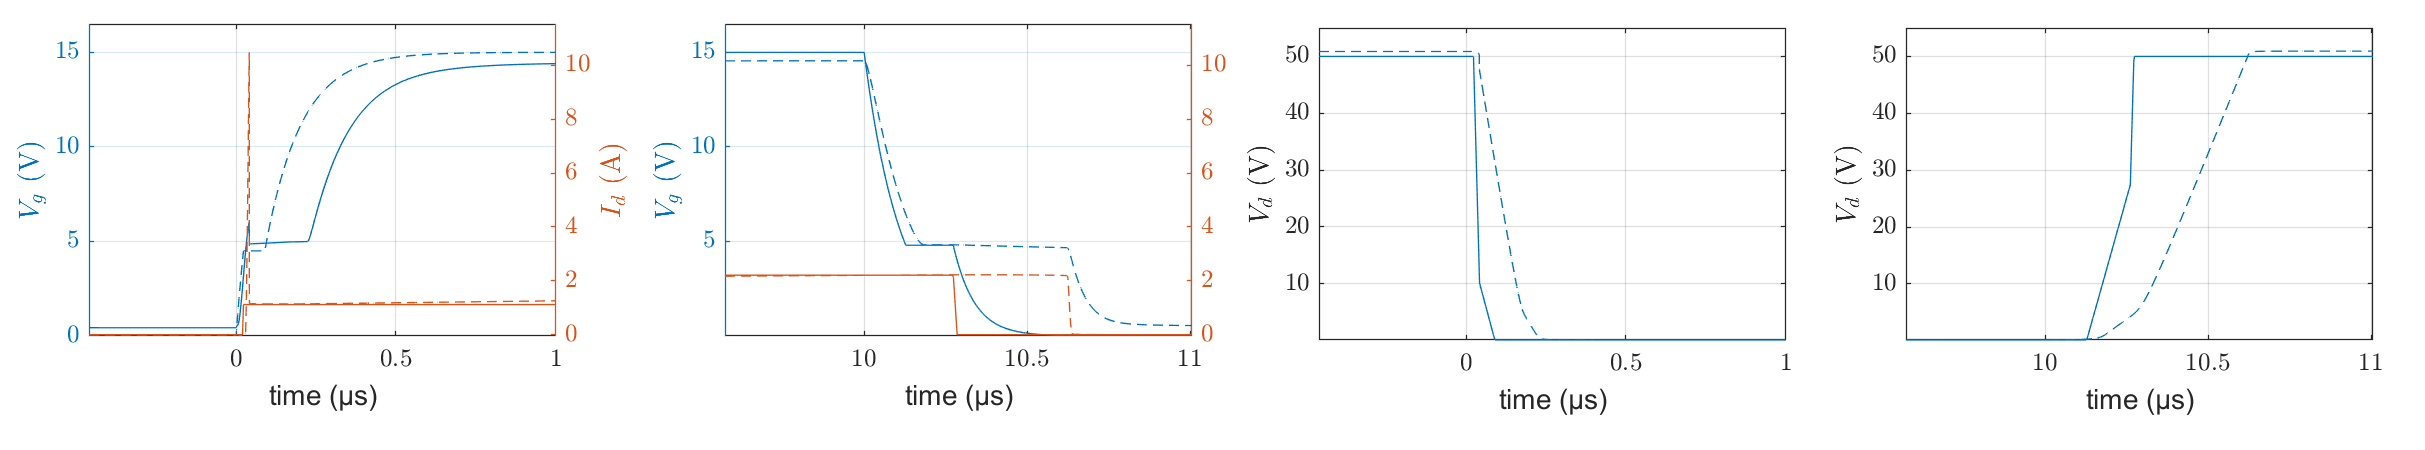
\includegraphics[width=0.7\linewidth]{images/ej1/comparison.png}
  \caption{Superposición de curvas simuladas (lineas sólidas) y obtenidas a partir de la teoría (lineas discontinuas). }
  \label{fig:comparison}
\end{figure}


\end{document}
